\documentclass[12pt]{article}

\usepackage{graphicx} %LaTeX package to import graphics
\graphicspath{{images/}} %configuring the graphicx package
 
% A project report typically consists of the following sections:

% Introduction: This section provides an overview of the project, including its background, objectives, and scope.

% Methodology: This section outlines the approach and methods used to carry out the project, including the research design, data collection, and analysis techniques.

% Results: This section presents the findings and outcomes of the project, including any data, charts, or graphs that support the conclusions.

% Discussion: This section discusses the implications of the results and how they contribute to the field or industry.

% Conclusion: This section summarizes the key points of the project and discusses any recommendations or next steps.

% References: This section lists all the sources cited in the report, following a specific citation style.

% Appendices: This section includes any additional materials that support the report, such as data sets or detailed calculations.



\title{\textbf{E-Commerce Subject Project}}
\author{\textbf{Book Selling Website}}

\begin{document}

\maketitle

\textbf{Team Members:}
\newline 
\textit{Dhruvkumar Patel, Kovil Savaj, Krunal Patel, and Manav Patel}


\newpage

\tableofcontents
\newpage

\section{Introduction}

\subsection{Abstract}

The e-commerce website for books is a \textbf{comprehensive online platform} for buying and selling books. It aims to provide a \textit{convenient and hassle-free} shopping experience to its customers by offering a wide range of books in different categories such as \textit{fiction, non-fiction, children's books, and more. }The website also allows users to browse through the books based on their \textit{interests and preferences,} and provides detailed descriptions and reviews for each book to help customers make informed purchase decisions. 

In addition to selling books, the website also offers a variety of other features to enhance the user experience. These include a \textit{wishlist function}, where customers can save their favorite books for later purchase, and a \textit{recommendation system,} which suggests similar books based on the customer's previous purchases. The website also provides a \textit{secure payment gateway and easy return policies} to ensure customer satisfaction.

\subsection{Methodology}

The methodology for the book selling e-commerce platform web project involved a combination of research, design, and development techniques.

To begin with, the team conducted market research to understand the needs and preferences of the target audience, as well as the competitive landscape of the industry. This included surveying book buyers and authors, and analyzing data on book sales and trends.

Based on the research findings, the team developed a wireframe and prototype of the platform, outlining the layout, functionality, and user experience. This was followed by user testing to gather feedback and make any necessary adjustments.

Next, the team designed and developed the front-end and back-end of the platform, using a combination of HTML, CSS, JavaScript, and a database management system. The platform was designed to be user-friendly and easy to navigate, with a clean and modern look. It was also optimized for mobile devices, allowing customers to shop on-the-go from their smartphones and tablets.

\newpage
\section{Diagrams}

\subsection{Use Case Diagram}

The use case diagram for the book selling e-commerce platform is a visual representation of the interactions between the various actors and the system. The actors in this context refer to the users of the platform, such as customers, authors, and administrators. The system refers to the e-commerce platform itself, including all the features and functionality it provides.

\begin{figure}[h]
\centering
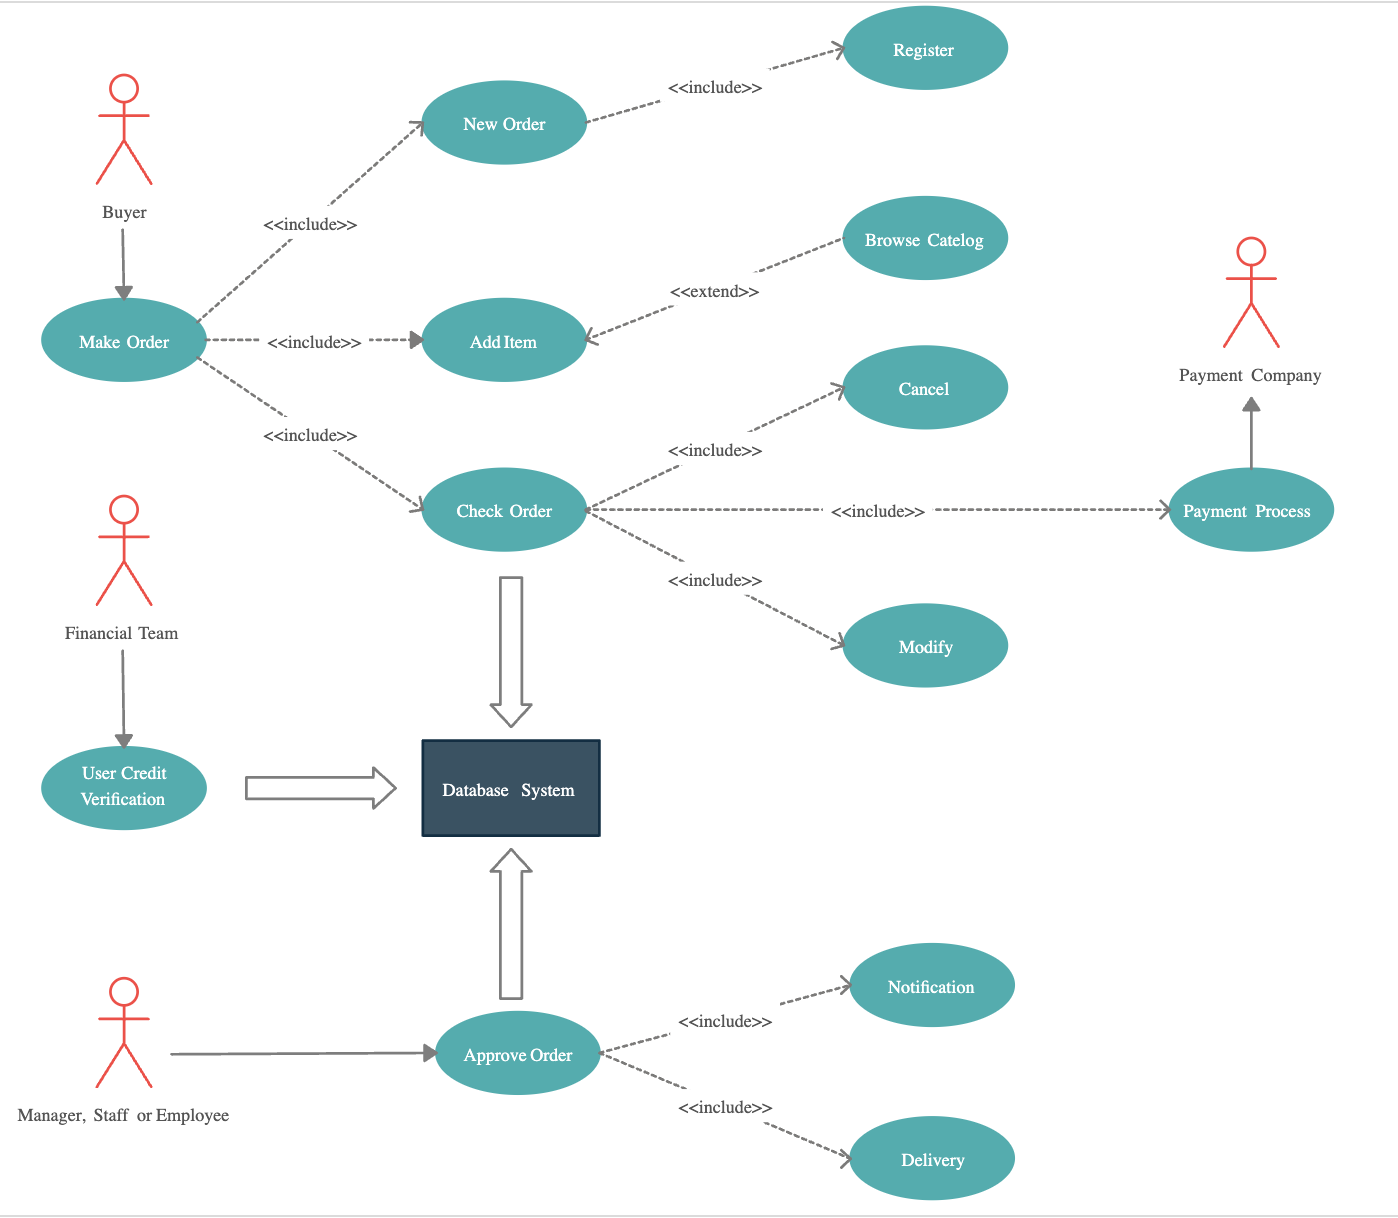
\includegraphics[width=0.85\textwidth]{use_case_diagram.png}
\caption{Use Case Diagram}
\end{figure}

The use case diagram shows the various actions that each actor can take within the system, as well as the outcomes of those actions. \textit{For example}, a customer can browse through the available books, and make a purchase. An administrator can manage the website, including approving and handling customer inquiries.

\newpage
\subsection{ER Diagram}

The ER (Entity Relationship) diagram for the entities of author, warehouse, customer, and publisher is a visual representation of the relationships between these entities within the e-commerce platform. The diagram shows how these entities are connected and interact with one another, as well as the attributes and properties that are associated with each entity.

\begin{figure}[h]
\centering
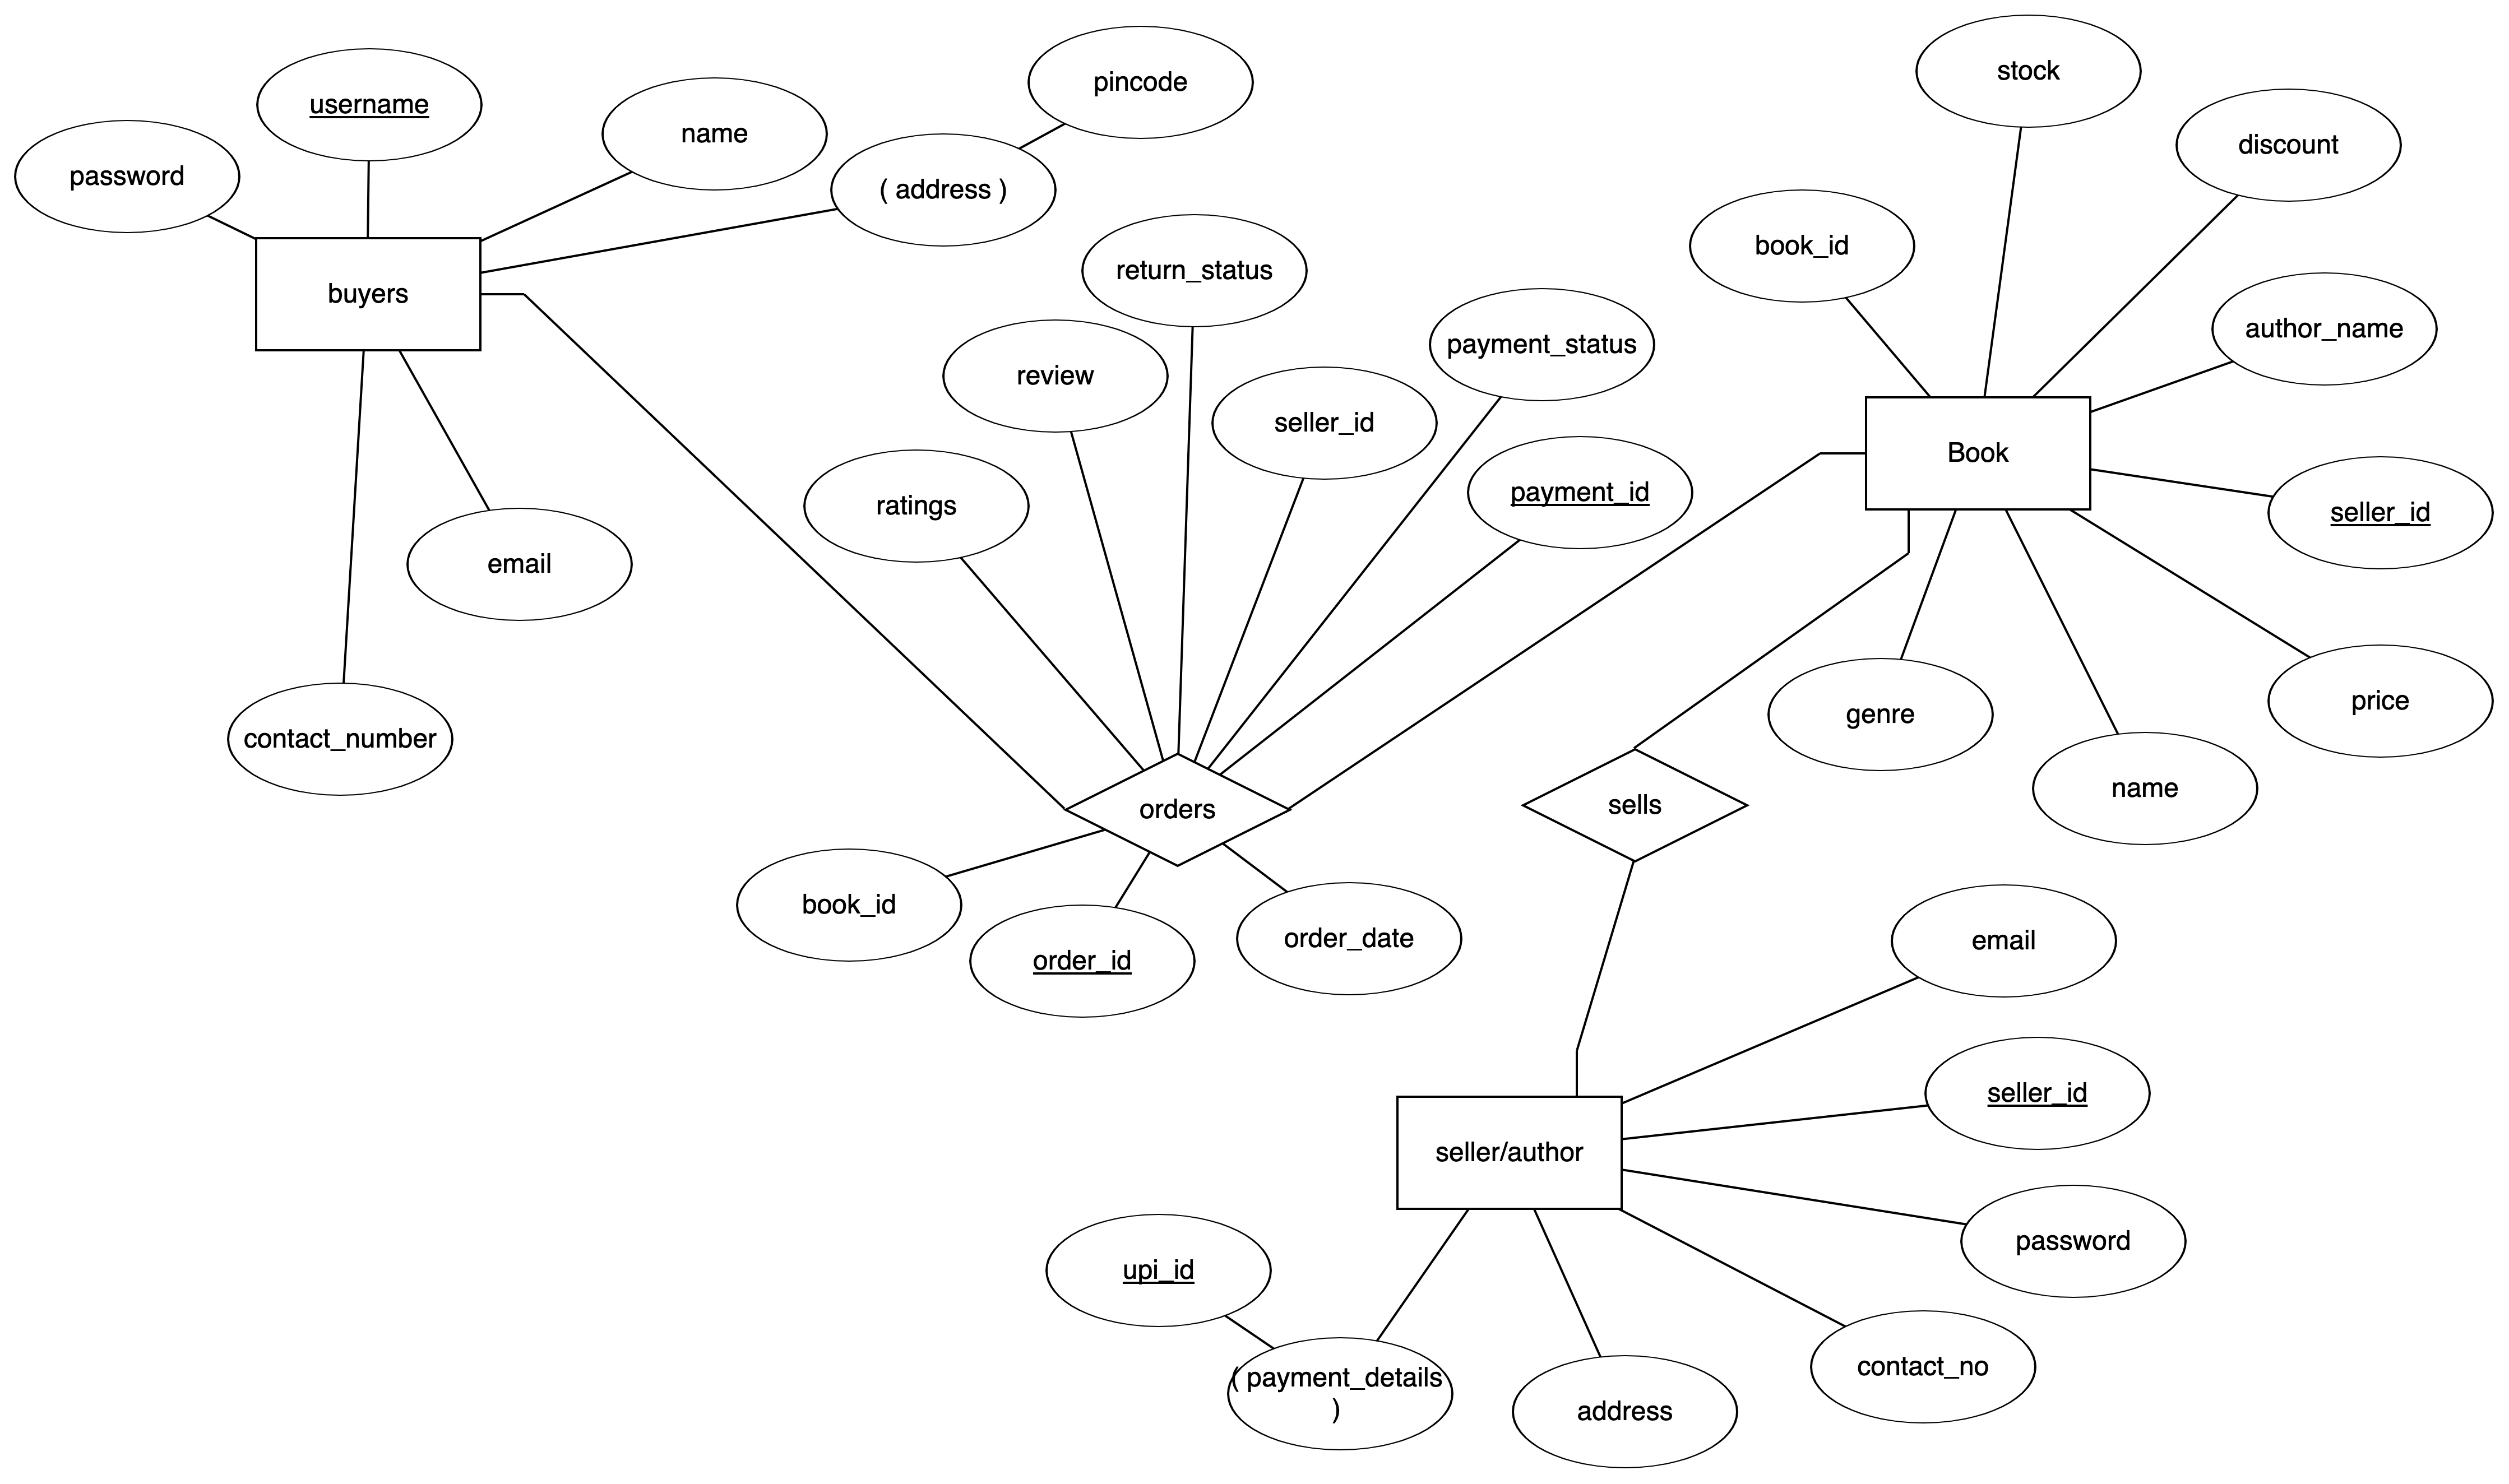
\includegraphics[width=0.85\textwidth]{er_diagram.png}
\caption{ER Diagram}
\end{figure}

\end{document}